\section{Evaluation}

We evaluate the implemented algorithm on doth regular and context-free path queries in order to demonstrate applicability of the proposed solution.
Namely, goals of the evaluation are following.
\begin{enumerate}
	\item Investigate practical applicability of RPQ evaluation by the proposed algorithm.
	\item Compare Azimov's algorithm for reachability CFPQ and the proposed algorithm.
	\item Investigate practical applicability of paths extraction algorithm for both regular and context-free queries.
\end{enumerate}

For evaluation, we use a PC with Ubuntu 18.04 installed.
It has Intel core i7-6700 CPU, 3.4GHz, and DDR4 64Gb RAM.
As far as we evaluate only algorithm execution time, we store each graph fully in RAM as its adjacency matrix in sparse format.
Note, that graph loading time is not included in the result time of evaluation.	

\subsection{RPQ Evaluation}

In oder to investigate applicability of the proposed algorithm for RPQ over real-world graphs we collect a set of real-world and synthetic graphs and evaluate queries generated by using the most popular templates for RPQs.

\subsubsection{Dataset}

Brief description of collected graphs are presented in table~\ref{tbl:graphs_for_rpq}.
Namely, the dataset consists of several parts.
The first one is a set of LUBM graphs\footnote{Lehigh University Benchmark (LUBM) web page: \url{http://swat.cse.lehigh.edu/projects/lubm/}. Access date: 07.07.2020.}~\cite{10.1016/j.websem.2005.06.005} with different number of vertices.
The second one is a graphs from Uniprot database\footnote{Universal Protein Resource (UniProt) web page: \url{https://www.uniprot.org/}. All files used for evaluation can be downloaded here: \url{ftp://ftp.uniprot.org/pub/databases/uniprot/current_release/rdf/}. Access date: 07.07.2020.}: \textit{proteomes}, \textit{taxonomy} and \textit{uniprotkb}.
The last part is a RDF files \textit{mappingbased\_properties} from DBpedia\footnote{DBpedia project web site: \url{https://wiki.dbpedia.org/}. Access date: 07.07.2020.} and \textit{geospecies}\footnote{The Geospecies RDF: \url{https://old.datahub.io/dataset/geospecies}. Access date: 07.07.2020.}.
These graphs represents data from different areas and they are frequently used for graph querying algorithms evaluation.

\begin{table}
\begin{tabular}{|l|c|c|}
\hline
Graph & \#V & \#E \\
\hline
\hline 
LUBM100  & 300000 & 4000000 \\
LUBM300  & 3 & 4 \\
LUBM500  & 3 & 4 \\
LUBM1M   & 3 & 4 \\
LUBM1.5M & 3 & 4 \\
LUBM1.9M & 3 & 4 \\
\hline
Uniprotkb & 3 & 4 \\
Proteomes & 3 & 4 \\
Taxonomy & 3 & 4 \\
\hline
Geospecies & 3 & 4 \\
Mappingbased\_properties & 3 & 4 \\
\hline
\end{tabular}
\caption{Graphs for RPQ evaluation}
\label{tbl:graphs_for_rpq}
\end{table}


Queries for evaluation was generated by using templates of the most popular RPQs which are collected from~
\cite{Pacaci2020RegularPQ} (Table 2) and~\cite{Wang2019} (some of complex queries from Table 5), and are presented in table~\ref{tbl:queries_templates}.
We generate 10 queries for each template and each graph using the most frequent relations from the given graph randomly\footnote{Used generator is available as part of CFPQ\_data project: \url{https://github.com/JetBrains-Research/CFPQ_Data/blob/master/tools/gen_RPQ/gen.py}. Access data: 07.05.2020.}. 
For all LUBM graphs common set of queries was generated in order to investigate scalability of the proposed algorithm.

\begin{table}
{\small
\begin{tabular}{|c|c||c|c|}
\hline

Name & Query & Name & Query \\
\hline
\hline 
q\_1    & $a^*$                               & q\_9\_5  & $(a \mid b \mid c \mid d \mid e)^+$                     \\
q\_2    & $a\cdot b^*$                        & q\_10\_2 & $(a \mid b) \cdot c^*$                                  \\
q\_3    & $a \cdot b^* \cdot c^*$             & q\_10\_3 & $(a \mid b \mid c)  \cdot d^*$                          \\
q\_4\_2 & $(a \mid b)^*$                      & q\_10\_4 & $(a \mid b \mid c \mid d)  \cdot e^*$                   \\
q\_4\_3 & $(a \mid b \mid c)^*$               & q\_10\_5 & $(a \mid b \mid c \mid d \mid e)  \cdot f^*$            \\
q\_4\_4 & $(a \mid b \mid c \mid d)^*$        & q\_10\_2 & $a \cdot b$                                             \\
q\_4\_5 & $(a \mid b \mid c \mid d \mid e)^*$ & q\_11\_3 & $a \cdot b \cdot c$                                     \\
q\_5    & $a \cdot b^* \cdot c$               & q\_11\_4 & $a \cdot b \cdot c \cdot d$                             \\
q\_6    & $a^* \cdot b^*$                     & q\_11\_5 & $a \cdot b \cdot c \cdot d \cdot f$                     \\
q\_7    & $a \cdot b \cdot c^*$               & q\_12    & $(a \cdot b)^+ \mid  (c \cdot d)^+$                     \\
q\_8    & $a? \cdot b^*$                      & q\_13    & $(a \cdot(b \cdot c)^*)^+ \mid  (d \cdot f)^+$          \\
q\_9\_2 & $(a \mid b)^+$                      & q\_14    & $(a \cdot b \cdot (c \cdot d)^*)^+  \cdot (e \mid f)^*$ \\
q\_9\_3 & $(a \mid b \mid c)^+$               & q\_15    & $(a \mid b)^+ \cdot (c \mid d)^+$                       \\
q\_9\_4 & $(a \mid b \mid c \mid d)^+$        & q\_16    & $a \cdot b \cdot (c \mid d \mid e)$                     \\
\hline
\end{tabular}
}
\caption{Graphs for RPQ evaluation}
\label{tbl:queries_templates}
\end{table}


\subsubsection{Results}

Results of evaluation

Reachability index creation time for each query for LUBM graphs set is presented in figure~\ref{fig:lubm_all_qs}.
We can observe linear dependency of evaluation time on graph size.
Also we can see, that query evaluation time depends on query: there are queries which evaluate less then 1 second even for biggest graph (q\_2, q\_5, q\_11\_2, q\_11\_3), while worst time is 6.26 seconds.
Anyway, we can argue that in this case our algorithm demonstrates reasonable time to be applied for real-world data analysis, because  !!!!

\begin{figure}
   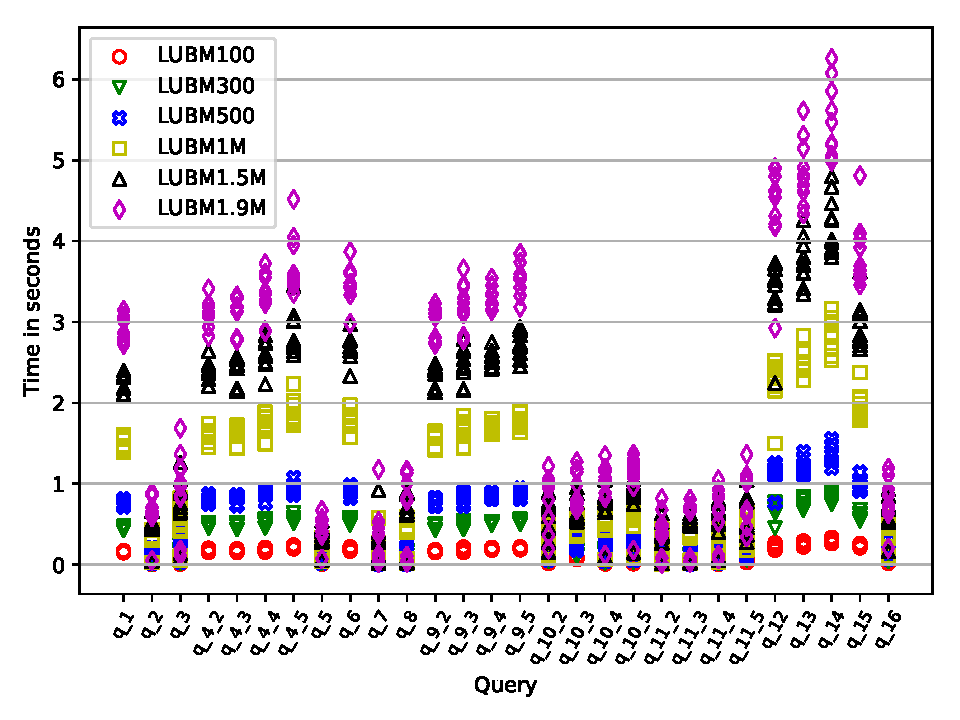
\includegraphics[width=0.48\textwidth]{data/LUBM_all.pdf}
   \caption{Reachability index creation time for LUBM series}
   \label{fig:lubm_all_qs}
\end{figure}


Reachability index creation time for each query for for real-world graphs is presented in figure~\ref{fig:other_all_qs}.

\begin{figure}
   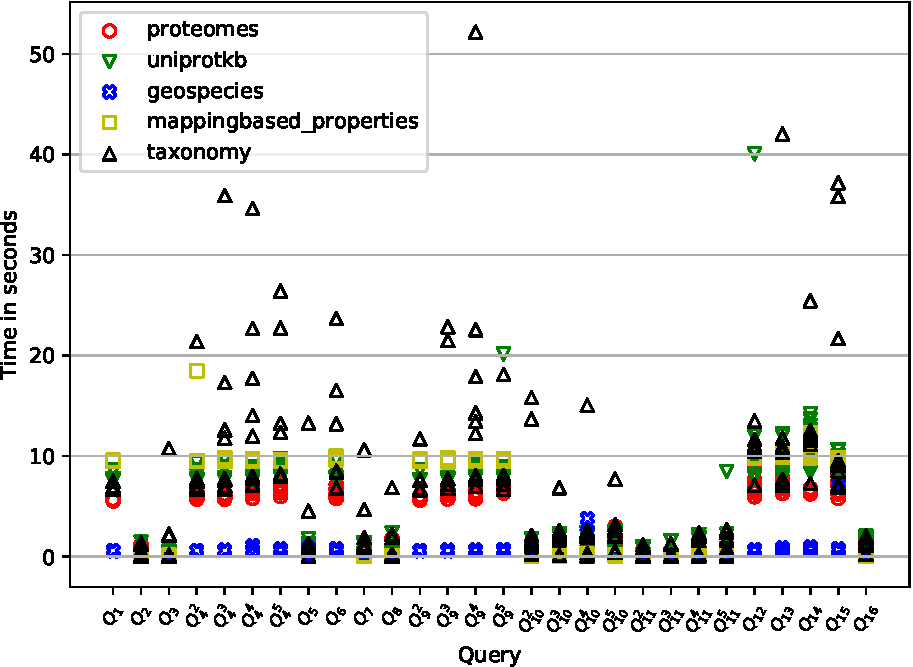
\includegraphics[width=0.48\textwidth]{data/other_all.pdf}
   \caption{Reachability index creation time for real-world RDFs}
   \label{fig:other_all_qs}
\end{figure}

Paths extraction was evaluated on cases with possible long paths.
These cases were selected during reachability index creation by using number of iterations in transitive closure evaluation.
For each selected graph and query we measure paths extraction time for each reachable pair. 

We evaluate two scenarios.
The first one is a single path extraction.
In this case results are represented as a dependency of extraction time on extracted path length.
We can see linear !!!!

The second scenario is many paths extraction.
Here we limit a number of path to extract by !!! 
In this case results are represented as a dependency of extraction time on number of extracted paths.


\begin{figure}
   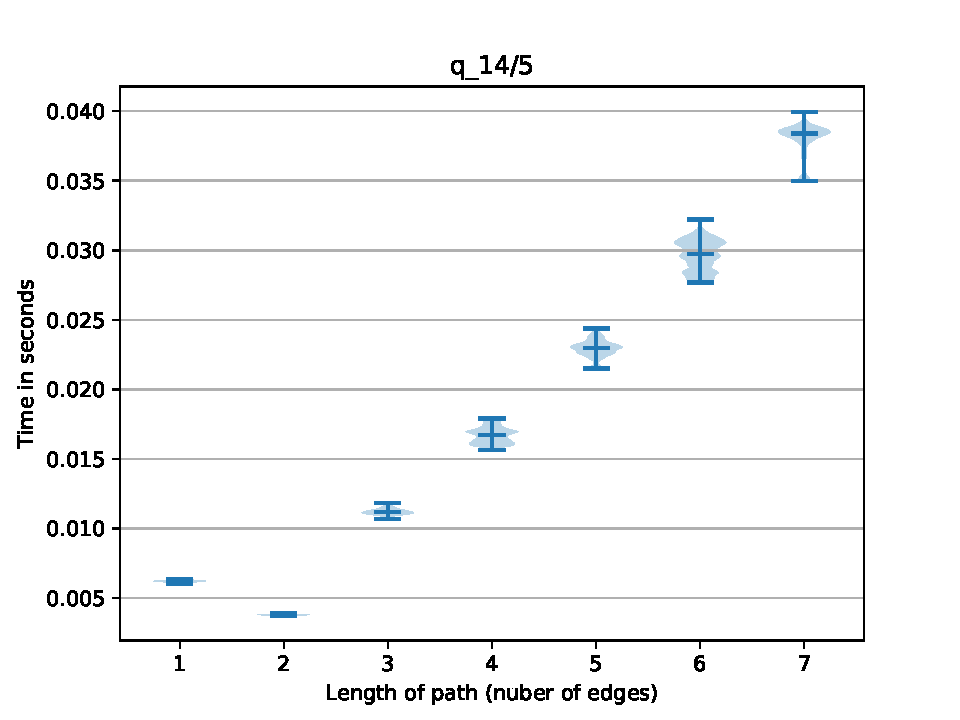
\includegraphics[width=0.48\textwidth]{data/res_graphics/q_14_5.pdf}
   \caption{Single path extraction}
\end{figure}



\subsubsection{Conclusion}

\subsection{CFPQ Evaluation}

Comparison with matrix-based algorithm.

\subsubsection{Dataset}

Dataset for evaluation. 
It should be CFPQ\_Data\footnote{CFPQ\_Data is a dataset for CFPQ evaluation which contains both synthetic and real-world data and queries \url{https://github.com/JetBrains-Research/CFPQ\_Data}. Access date: 07.07.2020.}

Same-generation queries, memory aliases.

\subsubsection{Results}

Results of evaluation.

Index creation.

Paths extraction.

\subsubsection{Conclusion}
